\section{Дуги, хорды и расстояния до центра}

\begin{wrapfigure}{r}{40mm}
\centering
\includegraphics{mppics/ris-120}
\caption{}\label{1938/ris-120}
\end{wrapfigure}

\paragraph{}\label{1938/109}
\mbox{\so{Теоремы}.}
\textbf{\emph{В одном круге или в равных кругах:}}

1) \textbf{\emph{если дуги равны, то стягивающие их хорды равны и одинаково удалены от центра.}}

2) \textbf{\emph{если две дуги, меньшие полуокружности, не равны, то б\'{о}льшая из них стягивается б\'{о}льшей хордой и из обеих хорд б\'{о}льшая расположена ближе к центру.}}

1) Пусть дуга $AB$ равна дуге $CD$ (рис.~\ref{1938/ris-120}), требуется доказать, что хорды $AB$ и $CD$ равны, а также равны перпендикуляры $OE$ и $OF$, опущенные из центра на хорды.

Повернём сектор $AOB$ вокруг центра $O$ в направлении, указанном стрелкой, на столько, чтобы радиус $OB$ совпал с $OC$.
Тогда дуга $BA$ пойдёт по дуге $CD$ и вследствие их равенства эти дуги совместятся.
Значит, хорда $AB$ совместится с хордой $CD$ и перпендикуляр $OE$ совпадёт с $OF$ (из одной точки можно опустить на прямую только один перпендикуляр), то есть
$AB=CD$ и $OE=OF$.

\begin{wrapfigure}{o}{40mm}
\centering
\includegraphics{mppics/ris-121}
\caption{}\label{1938/ris-121}
\end{wrapfigure}

2) Пусть дуга $AB$ (рис.~\ref{1938/ris-121}) меньше дуги $CD$, и притом обе дуги меньше полуокружности;
требуется доказать, что хорда $AB$ меньше хорды $CD$, а перпендикуляр $OE$ больше перпендикуляра $OF$.
Отложим на дуге $CB$ дугу $CK$, равную $AB$, и проведём вспомогательную хорду $CK$, которая, по доказанному, равна хорде $AB$ и одинаково с ней удалена от центра.
У треугольников $COD$ и $COK$ две стороны одного равны двум сторонам другого (как радиусы), а углы, заключённые между этими сторонами, не равны;
в этом случае, как мы знаем (§~\ref{1938/52}), против большего из углов, то есть
$\angle COD$, должна лежать б\'{о}льшая сторона;
значит, $CD>CK$, и потому $CD>AB$.

Для доказательства того, что $OE>OF$, проведём $OL\perp CK$ и примем во внимание, что, по доказанному, $OE=OL$;
следовательно, нам достаточно сравнить $OF$ с $OL$.
В прямоугольном треугольнике $OFM$ (покрытом на чертеже штрихами) гипотенуза $OM$ больше катета $OF$;
но $OL>OM$;
значит, и подавно $OL>OF$, и потому $OE>OF$.

Теорема, доказанная нами для одного круга, остаётся верной и для равных кругов, потому что такие круги один от другого отличаются только положением.

\paragraph{}\label{1938/110}
\so{Обратные теоремы}.
Так как в предыдущем параграфе рассмотрены всевозможные взаимно исключающие случаи относительно сравнительной величины двух дуг одного радиуса, причём получились взаимно исключающие выводы относительно сравнительной величины хорд и расстояний их от центра, то обратные предложения должны быть верны, а именно.

\textbf{\emph{В одном круге или в равных кругах:}}

1) \textbf{\emph{равные хорды одинаково удалены от центра и стягивают равные дуги;}}

2) \textbf{\emph{хорды, одинаково удалённые от центра, равны и стягивают равные дуги;}}

3) \textbf{\emph{из двух неравных хорд б\'{о}льшая ближе к центру и стягивает б\'{о}льшую дугу;}}

4) \textbf{\emph{из двух хорд, неодинаково удалённых от центра, та, которая ближе к центру, больше и стягивает б\'{о}льшую дугу.}}

Эти предложения легко доказываются от противного.
Например, для доказательства первого из них рассуждаем так:
если бы данные хорды стягивали неравные дуги, то, согласно прямой теореме, они были бы не равны, что противоречит условию;
значит, равные хорды должны стягивать равные дуги;
а если дуги равны, то, согласно прямой теореме, стягивающие их хорды одинаково удалены от центра.

\paragraph{}\label{1938/111}
\mbox{\so{Теорема}.}
\textbf{\emph{Диаметр есть наибольшая из хорд.}}

\begin{wrapfigure}{o}{40mm}
\centering
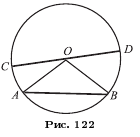
\includegraphics{mppics/ris-122}
\caption{}\label{1938/ris-122}
\end{wrapfigure}

Если соединим с центром $O$ концы какой-нибудь хорды, не проходящей через центр, например хорды $AB$ (рис.~\ref{1938/ris-122}), то получим треугольник $AOB$, в котором одна сторона есть эта хорда, а две другие — радиусы.
Но в треугольнике каждая сторона менее суммы двух других сторон;
следовательно, хорда $AB$ менее суммы двух радиусов, тогда как всякий диаметр $CD$ равен сумме двух радиусов.
Значит, диаметр больше всякой хорды, не проходящей через центр.
Но так как диаметр есть тоже хорда, то можно сказать, что диаметр есть наибольшая из хорд.
